\documentclass[11pt]{article}
\usepackage{fullpage}
\usepackage{amsmath}
\usepackage{amssymb}
\usepackage{graphicx} 
\usepackage{listings}
\usepackage{framed}
\usepackage{caption}
\usepackage{subcaption}
\usepackage{titling}
\usepackage{algorithm}
\usepackage{algorithmic}



\newcommand{\allactionset}{\mathbb{A}}

\renewcommand{\algorithmicrequire}{\textbf{Input:}}
\renewcommand{\algorithmicensure}{\textbf{Output:}}



\setlength{\droptitle}{-4em}     % Eliminate the default vertical space
\addtolength{\droptitle}{-22pt}   % Only a guess. Use this for adjustment

\title{ \bf
Object detection via Contextual Sequence Optimization - an alternative to non-max suppression
}

\date{}
\author{Shervin Javdani, Karthik Lakshmanan, Jiaji Zhou}



\begin{document}
\maketitle

\vspace{-15mm}

\section{Introduction}
We aim to build a system for detecting multiple instances of a target object in an image. In the current paradigm, a sliding window model is used, which slides a trained detector across the image, and scores each patch independently. A post-processing step known as non-maximal suppression is used to resolve dependencies between overlapping candidate windows. In this step, among all windows that overlap, only the one with the maximum score is retained and the others are discarded. However, this may be problematic - what if there were indeed multiple objects located there? Furthermore, we may expect that for some objects which tend to appear in groups, e.g. trees, having a detector fire actually provides more evidence that nearby patches are detecting trees. 

In this project, we will explore eliminating independence of the various sliding windows. In particular, we explore the use of using previous object detection decisions and scores to determine where to place the next detection window. The problem can then be formulated as - given windows $W_1 \ldots W_i$ with scores $S_1 \ldots S_i$, where should window $W_{i+1}$ be placed in order to maximize some scoring objective (Eg: Coverage). 

To do so efficiently, we will apply recent work on Contextual Sequence Prediction~\cite{dey_2012_conseqopt} and submodular function maximization. This works presents a simple, efficient, reduction-based approach where the choice and order of the items is established by repeatedly learning simple classifiers or regressors for each “slot” in a sequence. The key idea is that each “slot” takes into account the output of previous slots, attempting to maximize marginal benefit for that slot given previous outputs. In essence, subsequent slots will hold different “viewpoints”  from previous ones, therefore affecting their prediction. This approach leverages recent work on submodular function maximization to provide formal guarantees with respect to the optimal sequence, where a simple greedy approach can be used for training each slot.

\section{Dataset}

We hope to apply the above methods to detecting people, and are working with the INRIA Person dataset~\cite{HoG}. The dataset includes full images, with bounding box annotations for individual people. We have setup the infrastructure for reading in these images and annotations, but have not tied this framework into the training.

\section{Image features}

In order to detect people in images, we are using the Histogram of Oriented Gradients (HOG) as feature descriptors. These descriptors were first used by Dalal and Triggs \cite{HoG} to detect humans in 2D images. The key idea behind the Histogram of Oriented Gradient descriptors is that local object appearance and shape within an image can be described by the distribution of intensity gradients or edge directions. To compute these features, the image is divided into small connected regions, called cells, and for each cell we compile a histogram of gradient directions or edge orientations for the pixels within the cell. The combination of these histograms then represents the descriptor. For improved accuracy, the local histograms can be contrast-normalized by calculating a measure of the intensity across a larger region of the image, called a block, and then using this value to normalize all cells within the block. This normalization results in better invariance to changes in illumination or shadowing.

An Integral Histogram representation, presented by Porikli \cite{IntHist} can be used for fast calculation of HoG features over arbitrary rectangular regions of the image, as it is computationally efficient. This technique exploits the spatial arrangement of data points, and recursively propagates an aggregated histogram by starting from the origin and traversing through the remaining points along either a scan-line or a wave-front. At each step, a single bin is updated using the values of integral histogram at the previously visited neighboring data points. After the integral histogram is propagated, histogram of any target region can be computed easily by using simple arithmetic operations.

We are using a C++ implementation of a HoG feature extractor that uses Integral Histograms, and was developed by Liang-Liang He. We are currently able to extract a vector HoG features for any given rectangular window. We are currently using 8 orientation bins and a cell size of 4x4 pixels. We will continue to tune these parameters for better detection of people in images.


\section{Utility Function}
One key requirement for ConSeqOpt is that the utility function is both \emph{monotone} and \emph{submodular}. Let $\allactionset$ be the set of all actions currently available at this time (windows we can place our detector). We call a function $f$ submodular if whenever $X \subseteq Y \subseteq \allactionset$, $a \in \allactionset \backslash Y$:

\textbf{Submodularity} (diminishing returns):
\begin{align*}
  f(X \cup \{a\}) - f(X) \geq f(Y \cup \{a\}) - f(Y)
\end{align*}

The marginal benefit of adding $a$ to a smaller set $X$ is at least as much as adding it to the superset $Y$. We also require monotonicty, or that adding more elements never hurts:

\textbf{Monotonicity} (more never hurts):
\begin{align*}
f(X \cup \{a\}) - f(X) \geq 0
\end{align*}

We believe we have come up with an objective that accomplishes our objective (finding people in images, with people at different scales) while satisfying these requirements. Essentially, we take each ground truth label of a person, and assign it to a specific scale at which it can be detected, depending on how large the person is in the image. Let $G = \{ (x_g,y_g,s_g)\}$ be the set of pixel locations and scales which were labeled as including a person (so the interior of a labeled region, assigned to a specific scale). See Figure~\ref{fig:pyramid} for an example.

Let $\allactionset$ be the set of 3-tuples $(x,y,s)$, corresponding to a position and scale we may place our detection window. Note that the window itself is of fixed size - the scale $s$ corresponds to the scale of the image in our pyramid. For an action $a \in \allactionset$, we note all pixels ``covered'' by the window with $C(a) = \{(x_a, y_a, s_a)\}$. We can also consider the total pixels covered by a set of actions $A \subseteq \allactionset$ as $C(A) = \cup_{a \in A} C(a)$. Our utility function over a set of actions is just the total number of pixels in $G$ that are covered by the union of actions in $A$, or:
\begin{align*}
  f_G(A) &= | C(A) \cap G|
\end{align*}

This is essentially the classic set-cover problem, which has been shown to be monotone submodular. A more rigorous proof will be included in our final report.

\begin{figure}
  \centering
  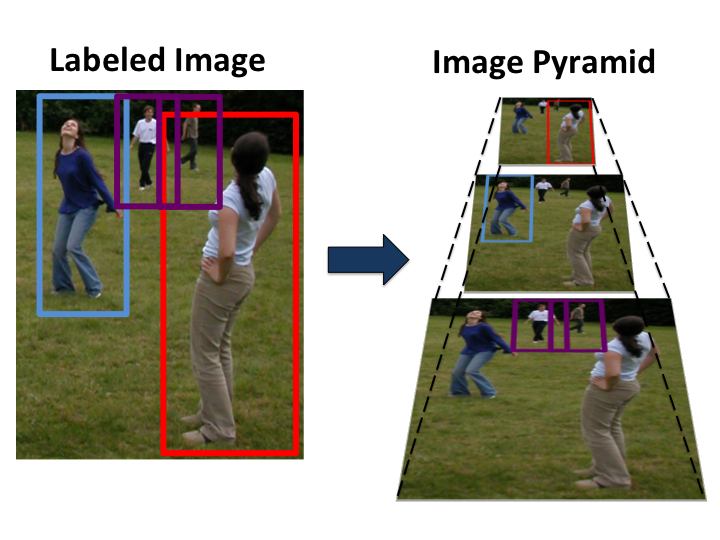
\includegraphics[trim=0 40 0 40, clip=true, width=0.7\columnwidth]{./images/pyramid.png} 
  \caption{We take our labeled images, assign a scale to each label, and define a utility as how much of each labeled person we ``cover'' at that specific scale.}
  \label{fig:pyramid}
\end{figure}



\section{Ranking-based ConSeqOpt}
Algorithm~\ref{algorithm:ConSeqOpt} shows the pseudo-code for training Ranking-based ConSeqOpt
 \begin{figure*}[htb!]
  \begin{minipage}[t]{\textwidth}
    \begin{algorithm}[H]
      \caption{Algorithm for training \textsc{ConSeqOpt} using
          ranking machines}
      \label{conseqopt.rank}
      \begin{algorithmic}[1]
        \REQUIRE \texttt{Maximum number of windows $N$, Ranking Machine
          $\Re$, dateset $D$ of $|D|$ number of images, each with $|W_i|$ number of candidate windows}
        \ENSURE \texttt{sequence of ranking machines $\Re_1, \Re_2, \ldots, \Re_N$}
        \FOR{$i = 1$ \TO $N$} \label{reg.line1}
        \STATE $\Re_i \leftarrow \{\}$
        \FOR{$j = 1$ \TO $|D|$}
        \STATE $\mathbf{X_i^j}, \mathbf{M_{B_i}^j} \leftarrow \texttt{computeFeatures\&MarginalUnitGain}(D^j,\mathbf{Y^j_{\Re_1,\Re_2,\ldots,\Re_{i-1}}}, W_j)$ \label{reg.line2}
        \STATE $\Re_i \leftarrow \Re_i \cup \texttt{train}(\mathbf{X_i^j}, \mathbf{M^j_{B_{i}}})$ \label{reg.line3}
        \ENDFOR
        
        \FOR{$j = 1$ \TO $|D|$}
        \STATE $\mathbf{\tilde{M}^j_{B_i}} \leftarrow \texttt{rank}(\mathbf{X^j_i}, \Re_i)$ \label{reg.line4}
        \STATE $\mathbf{Y_{\Re_i}^j} = \texttt{argmax$_{k\in W_j}$}(\mathbf{\tilde{M}^j_{B_k}})$ \label{reg.line5}
         \ENDFOR \label{reg.line6}
        \ENDFOR 
     
      \end{algorithmic}
      \label{algorithm:ConSeqOpt}
    \end{algorithm}
  \end{minipage}
  \hfill
\end{figure*}
   
   We now further describe the training process for placing the $i$th window (for-loop $i$): 
   \begin{enumerate}
   \item Given all the previous chosen windows for all image$_j$ $\mathbf{Y^j_{\Re_1,\Re_2,\ldots,\Re_{i-1}}}$ $(j = 1,2,3...|D|)$, update the feature for all windows across all image$_j$ by updating the term of similarity to chosen sentences $\mathbf{Y^j_{\Re_1,\Re_2,\ldots,\Re_{i-1}}}$ in the feature vector. Then compute the marginal unit gain $\mathbf{M^j_{B_i}}$;   
   \item Rank the windows within each image$_j$ according to $\mathbf{M^j_{B_i}}$ and train a ranking machine $\Re_i$ (RankingSVM with slack variable weights proportional to pairwise difference in marginal unit gain); (lines 3-6)
   
   \item Based the trained ranking machine $\Re_i$, re-rank all windows $W_j$ for each image$_j$ and compute new ranking scores $\mathbf{\tilde{M}^j_{B_i}}$; 
   \item Foreach image$_j$, pick its top ranking sentence, denoted as $\mathbf{Y_{\Re_i}^j}$; (lines 7-10)
   \item Move to the next round i+1.   
   \end {enumerate}



\section{Next Steps}

Thus far, we have completed an implementation of Ranking-based ConSeqOpt for 1 round ($N=1$). We utilize Vowpal Wabbit~\cite{vw} for learning the svm ranking machine through adaptive online gradient descent. We are currently tying this in with our HoG descriptor code, computed over random patches from the INRIA dataset~\cite{HoG}, and extending the training to further rounds. One key question is what features can we incorporate from the previously selected windows (e.g. distance to nearest window).


\bibliographystyle{plain}
\bibliography{refs}


\end{document}
